\documentclass[a4paper, top=10mm]{article}
%for writing from the top
\usepackage{fullpage}
%for math
\usepackage{amsmath}
\usepackage{mathrsfs}
\usepackage{amsthm}
%for images
\usepackage{graphicx}
%for color
\usepackage{xcolor}
%for title
\title{\textbf{\huge{Mathematicians' Digital Clock}}}
\author{Enigma n\textsuperscript{o}3}
\date{19\textsuperscript{th} December 2024}

\newtheorem*{hint}{Hint}

\addtolength{\voffset}{-2cm}
\addtolength{\textheight}{5cm}


\begin{document}
	\maketitle
	
	A digital clock continuously displays four digits: two for the hours and two for the minutes, in a 24-hour format (from 00:00 to 23:59).
	
	During the Christmas party, mathematicians have agreed that the number four is the best one (because $2 + 2 = 2 \times 2 = 4$).
	Mathematicians are happy if at least one four appear on the digital clock.
	
	How many minutes a day are mathematicians happy?
	
	I.e.: In a day, for how many minutes does the digit 4 appear at least once on the clock?
	
	\begin{center}
		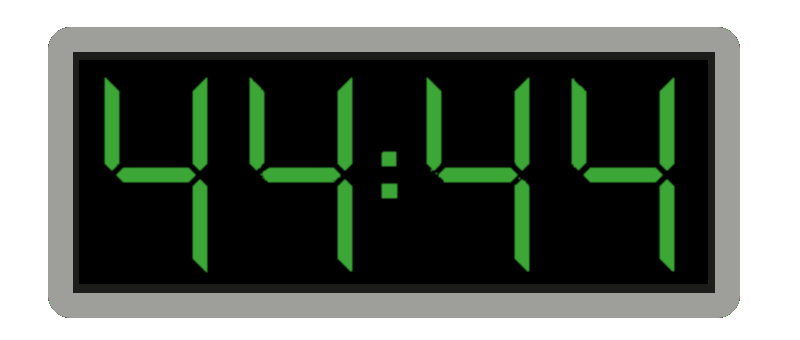
\includegraphics[width=\linewidth]{03clock.png}\\
		Digital clock making mathematicians \textit{very} happy.
	\end{center}
	
	% Answer: we count new minutes for each digit
	% left digit: 0
	% middle left digit: 2h = 120 min
	% middle right digit: 10min * 22 = 220min
	% right digit: 5min * 22 = 110min
	% => 450min
	
\end{document}